\chapter{RMN do próton}\label{ch:g12:proton-nmr}

Num hospital, um paciente está deitado dentro do anel de um aparelho de
ressonância magnética, e uma imagem dos tecidos \omterm{def:g10:the-mole:amount}{moles} do corpo aparece na
tela, construída a partir das respostas dos \omterm{def:g9:inside-the-atom:nucleus}{núcleos} de hidrogênio da sua
água e das suas gorduras. Num laboratório de química, um tubinho de
vidro com alguns miligramas de um composto é baixado no interior de um
ímã potente, e aparece um espectro construído do mesmo jeito: um ímã
forte, um sinal de rádio e \omterm{def:g9:inside-the-atom:nucleus}{núcleos} de hidrogênio que respondem a ele. No
espectrômetro do químico, cada \omterm{def:g9:inside-the-atom:nucleus}{núcleo} de hidrogênio responde de um jeito
um pouco diferente conforme os seus vizinhos, e o espectro é um mapa dos
\omterm{def:g7:atoms-and-molecules:atom}{átomos} de hidrogênio da \omterm{def:g7:atoms-and-molecules:molecule}{molécula}.

\begin{recall}
Um \omterm{def:g11:infrared:spectrum}{espectro infravermelho} mostra que ligações uma \omterm{def:g7:atoms-and-molecules:molecule}{molécula} contém
(\cref{ch:g11:infrared}). \omterm{def:g11:functional-groups:functional-group}{Grupos funcionais}, funções e \omterm{def:g11:organic-skeletons:isomer}{isômeros}
(\cref{ch:g11:functional-groups}, \cref{ch:g11:organic-skeletons}).
\end{recall}

\begin{omfigure}
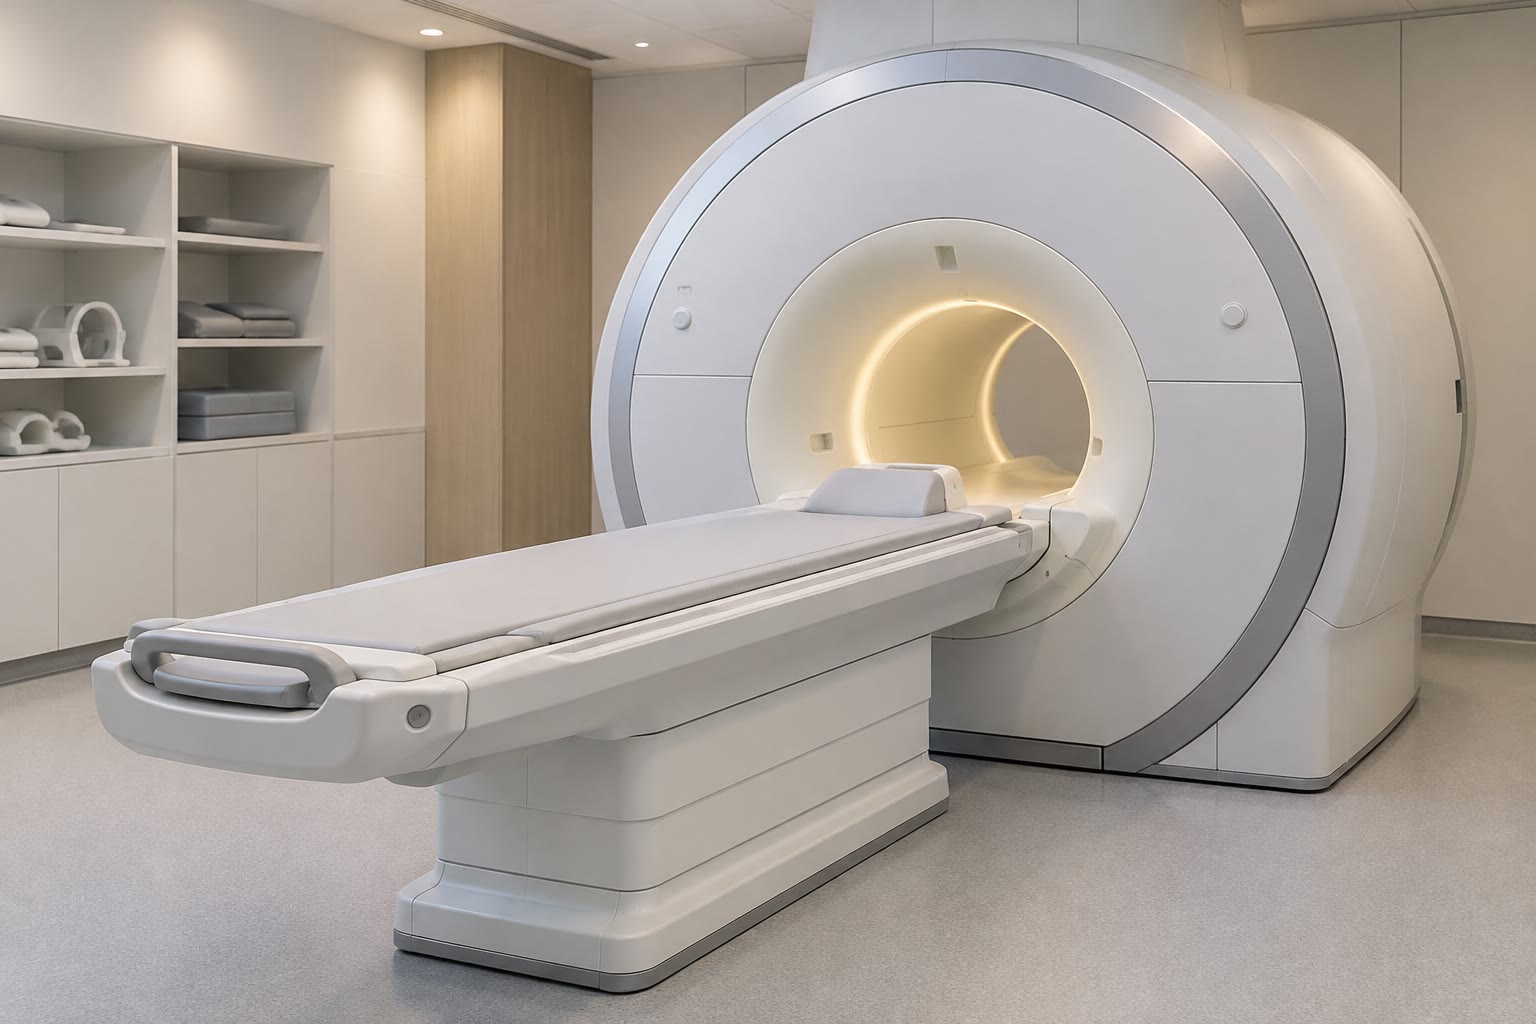
\includegraphics[width=0.48\linewidth]{images/book1/ai/g12-mri-room.jpg}

{\small Um aparelho de ressonância magnética: a mesma física do
espectrômetro de RMN do químico.}
\end{omfigure}

\section{Prótons num campo magnético}

O \omterm{def:g9:inside-the-atom:nucleus}{núcleo} de um \omterm{def:g7:atoms-and-molecules:atom}{átomo} de hidrogênio é um único \omterm{def:g9:inside-the-atom:proton}{próton}. Colocado num campo
magnético forte, ele absorve ondas de rádio de uma frequência precisa;
como e por quê é assunto da física, e não é necessário aqui. O que
importa ao químico é que os \omterm{def:g9:inside-the-atom:nucleus}{elétrons} em volta de um \omterm{def:g9:inside-the-atom:proton}{próton} o blindam um
pouco do campo, e que essa blindagem depende dos \omterm{def:g7:atoms-and-molecules:atom}{átomos} próximos: um
\omterm{def:g9:inside-the-atom:proton}{próton} vizinho de um \omterm{def:g7:atoms-and-molecules:atom}{átomo} de oxigênio eletronegativo, que puxa os
\omterm{def:g9:inside-the-atom:nucleus}{elétrons}, absorve numa frequência um pouco diferente da de um \omterm{def:g9:inside-the-atom:proton}{próton} de
uma cadeia de hidrocarboneto. As diferenças são minúsculas, alguns
milionésimos da frequência, e são dadas em partes por milhão.

\begin{omfigure}
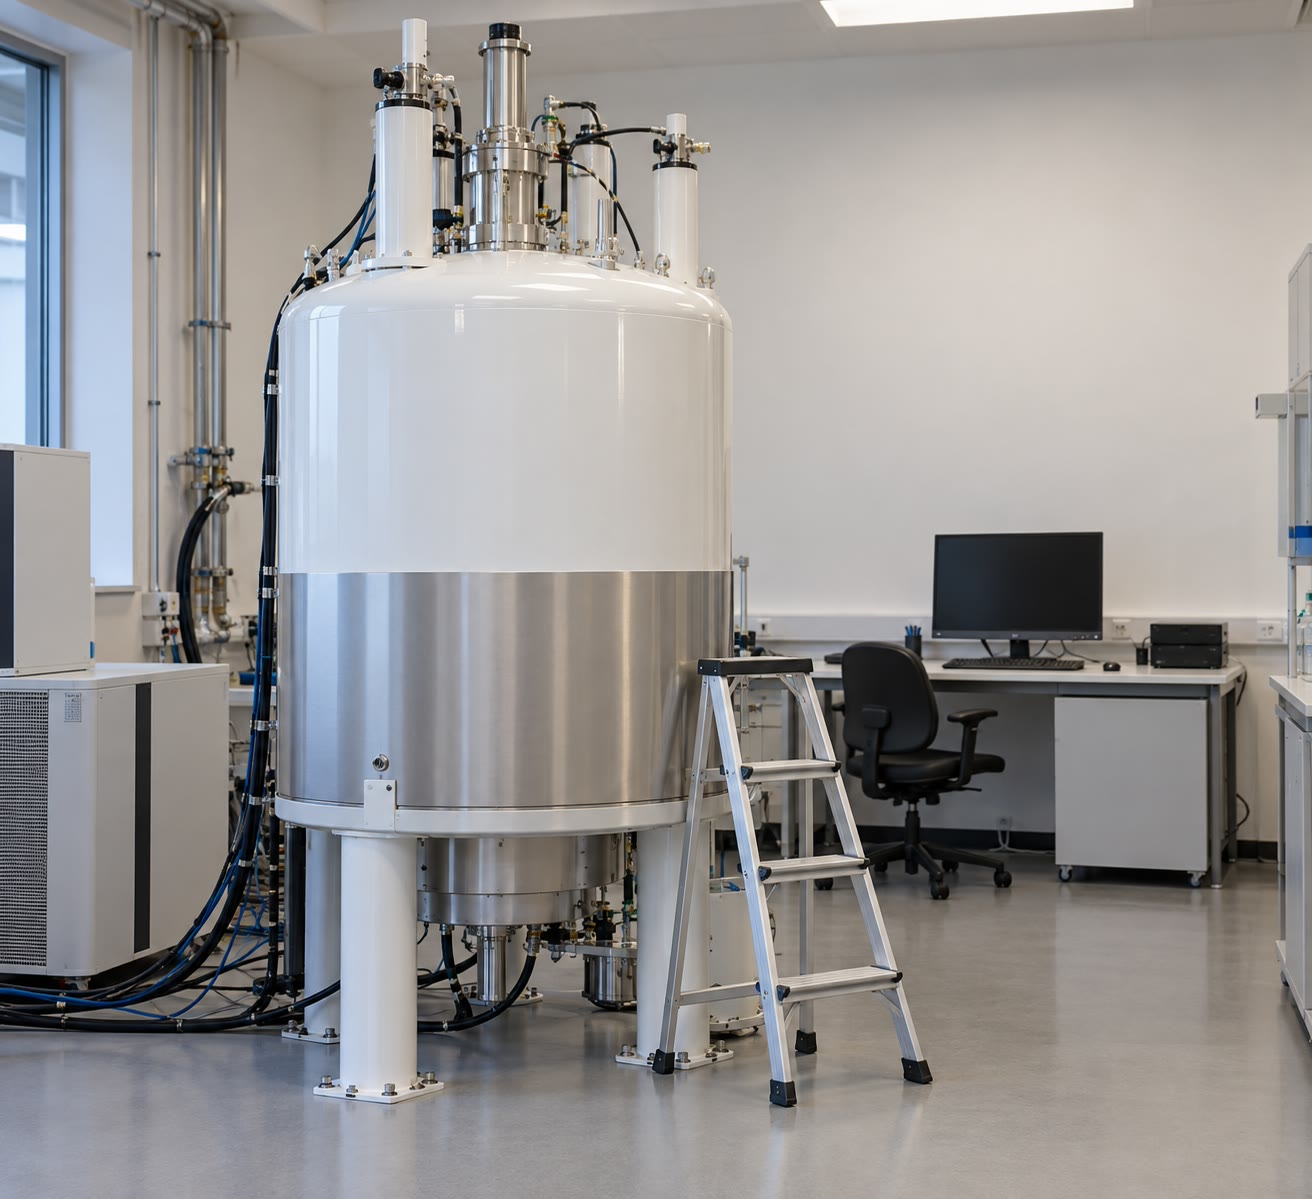
\includegraphics[width=0.42\linewidth]{images/book1/ai/g12-nmr-magnet.jpg}

{\small O ímã de um espectrômetro de RMN.}
\end{omfigure}

\begin{definition}[Espectro de RMN, deslocamento químico]\label{def:g12:proton-nmr:spectrum}
Um \emph{espectro de RMN}\index{espectro de RMN} do \omterm{def:g9:inside-the-atom:proton}{próton} (ressonância
magnética nuclear) mostra os sinais absorvidos pelos \omterm{def:g9:inside-the-atom:nucleus}{núcleos} de
hidrogênio de um composto. A posição de um sinal é o seu
\emph{deslocamento químico}\index{deslocamento quimico@deslocamento químico} $\delta$, em
partes por milhão (\si{ppm}), medido a partir do sinal de um composto de
referência, o tetrametilsilano \ce{Si(CH3)4} (TMS), fixado em
$\delta = 0$. O eixo de $\delta$ é desenhado crescendo da direita para a
esquerda.
\end{definition}

\begin{proposition}[O deslocamento depende dos vizinhos]\label{prop:g12:proton-nmr:shift}
% ledger: nmrr:CH3, nmrr:CH2, nmrr:allylic, nmrr:ketone, nmrr:halide, nmrr:alcohol, nmrr:vinylic, nmrr:aryl, nmrr:aldehyde, nmrr:acid
O \omterm{def:g12:proton-nmr:spectrum}{deslocamento químico} de um \omterm{def:g9:inside-the-atom:proton}{próton} depende dos \omterm{def:g7:atoms-and-molecules:atom}{átomos} próximos dele:
quanto mais perto ele está de um \omterm{def:g7:atoms-and-molecules:atom}{átomo} eletronegativo ou de uma \omterm{def:g10:lewis-and-shape:multiple-bond}{ligação
dupla}, maior é o seu deslocamento. Faixas típicas, em \si{ppm}:
\begin{center}
\small
\begin{tabular}{ll@{\qquad}ll}
\hline
ambiente & $\delta$ & ambiente & $\delta$ \\
\hline
\ce{CH3} numa cadeia & 0.7--1.3 & \ce{H-C-O} (\omterm{def:g11:functional-groups:alcohol}{álcool}, éter, \omterm{def:g11:functional-groups:carboxylic-acid}{éster}) & 3.3--4.5 \\
\ce{CH2} numa cadeia & 1.2--1.6 & \ce{H-C=C} & 4.5--6.5 \\
\ce{H-C-C=C} & 1.6--2.2 & H num anel benzênico & 6.5--8.0 \\
\ce{H-C-C=O} & 2.0--2.4 & \omterm{def:g11:functional-groups:carbonyl}{aldeído} \ce{-CHO} & 9.7--10.0 \\
\ce{H-C-X} (\omterm{def:g10:electron-shells:family}{halogênio}) & 2.5--4.0 & ácido \ce{-COOH} & 11.0--12.0 \\
\hline
\end{tabular}
\end{center}
\end{proposition}

\begin{proof}
Medido em muitos compostos. Um vizinho
eletronegativo atrai os \omterm{def:g9:inside-the-atom:nucleus}{elétrons} para longe do \omterm{def:g9:inside-the-atom:proton}{próton}, que fica menos
blindado e absorve num deslocamento maior.
\end{proof}

\begin{omfigure}
\begin{tikzpicture}[font=\small, x=0.75cm, y=0.5cm]
  % delta axis reversed: x = 12 - delta
  \draw[->] (0,0) -- (12.4,0) node[right] {};
  \foreach \d in {12,11,10,9,8,7,6,5,4,3,2,1,0}
    \draw ({12-\d},0) -- ({12-\d},-0.2) node[below, font=\footnotesize] {\d};
  \node[below=14pt] at (6,-0.3) {$\delta$ (\si{ppm})};
  \foreach \a/\b/\y/\c/\l in {
      11.0/12.0/1/omThm/{\ce{COOH}},
      9.7/10.0/2/omThm/{\ce{CHO}},
      6.5/8.0/1/black!60/{anel benzênico},
      4.5/6.5/2/omMeth/{\ce{C=C-H}},
      3.3/4.5/3/omDef/{\ce{H-C-O}},
      2.0/2.4/4/omProp/{\ce{H-C-C=O}},
      0.7/1.6/5/black!45/{\ce{CH3}, \ce{CH2} de cadeias}} {
    \fill[\c, rounded corners=1pt] ({12-\b},{\y-0.3}) rectangle ({12-\a},{\y+0.3});
    \node[anchor=west, font=\footnotesize] at ({12-\a+0.1},\y) {\l};
  }
  \draw[thick] (12,0) -- (12,0.6) node[above, font=\footnotesize] {TMS};
\end{tikzpicture}

{\small Onde os \omterm{def:g9:inside-the-atom:proton}{prótons} absorvem, por ambiente. Os \omterm{def:g9:inside-the-atom:proton}{prótons} próximos de um
oxigênio, de uma \omterm{def:g10:lewis-and-shape:multiple-bond}{ligação dupla} ou de um grupo ácido aparecem à esquerda
do espectro.}
\end{omfigure}

\begin{inthelab}[Preparar um tubo de RMN]
Alguns miligramas do composto são dissolvidos em cerca de
\qty{0.6}{mL} de um \omterm{def:g6:solutions-and-solubility:solute}{solvente} cujos \omterm{def:g7:atoms-and-molecules:atom}{átomos} de hidrogênio foram
substituídos por deutério (\ce{CDCl3}, clorofórmio deuterado), que não
dá nenhum sinal; acrescenta-se um traço de TMS como referência. A
solução é filtrada para dentro de um tubo de vidro fino, que é tampado,
etiquetado e baixado no ímã.
\end{inthelab}

\section{Prótons equivalentes}

\begin{definition}[Prótons equivalentes]\label{def:g12:proton-nmr:equivalent}
\omterm{def:g9:inside-the-atom:proton}{Prótons} são \emph{prótons equivalentes}\index{protons equivalentes@prótons equivalentes} se
eles têm o mesmo ambiente na \omterm{def:g7:atoms-and-molecules:molecule}{molécula}, de modo que absorvem no mesmo
deslocamento. Cada grupo de \omterm{def:g9:inside-the-atom:proton}{prótons} equivalentes dá um sinal. Os três
\omterm{def:g9:inside-the-atom:proton}{prótons} de um grupo \ce{CH3} são sempre equivalentes.
\end{definition}

\begin{example}[Contar os grupos]\label{ex:g12:proton-nmr:groups}
A propanona, \ce{CH3-CO-CH3}, tem seis \omterm{def:g9:inside-the-atom:proton}{prótons} mas um só grupo: os dois
\ce{CH3} são iguais, um de cada lado do \ce{C=O}. O etanol,
\ce{CH3-CH2-OH}, tem três grupos (\ce{CH3}, \ce{CH2}, \ce{OH}), e o
etanoato de etila, \ce{CH3-CO-O-CH2-CH3}, também três: o \ce{CH3}
vizinho do \ce{C=O}, o \ce{CH2} vizinho do \ce{O}, e o \ce{CH3} da
ponta.
\end{example}

\section{A integração}

\begin{definition}[Curva de integração]\label{def:g12:proton-nmr:integration}
A \emph{curva de integração}\index{curva de integracao@curva de integração} de um \omterm{def:g12:proton-nmr:spectrum}{espectro
de RMN} é uma curva, desenhada acima dos sinais, que sobe um degrau em
cada sinal: a altura de cada degrau é proporcional ao número de \omterm{def:g9:inside-the-atom:proton}{prótons}
que dão esse sinal.
\end{definition}

\begin{example}[Ler os degraus]\label{ex:g12:proton-nmr:steps}
No espectro do etanol, os degraus acima dos três sinais medem 2, 1 e 3
unidades, da esquerda para a direita: \ce{CH2}, \ce{OH} e \ce{CH3}. Só
as razões contam: degraus de 12, 6 e 18 mm dizem a mesma coisa.
\end{example}

\section{A multiplicidade e a regra do \texorpdfstring{$n+1$}{n+1}}


\begin{definition}[Multipleto, regra do $n+1$]\label{def:g12:proton-nmr:multiplet}
Um sinal muitas vezes é desdobrado em várias linhas próximas: um
\emph{multipleto}\index{multipleto} (singleto, dupleto, tripleto,
quarteto, \dots{} para 1, 2, 3, 4 linhas). Pela \emph{regra do
$n+1$}\index{regra do n+1@regra do $n+1$}, um grupo de \omterm{def:g12:proton-nmr:equivalent}{prótons
equivalentes} cujos \omterm{def:g7:atoms-and-molecules:atom}{átomos} de carbono vizinhos carregam ao todo $n$
\omterm{def:g9:inside-the-atom:proton}{prótons}, não equivalentes a ele, dá um sinal de $n+1$ linhas, com
intensidades nas razões do triângulo de Pascal.
\end{definition}

\begin{proposition}[O desdobramento pelos vizinhos]\label{prop:g12:proton-nmr:n-plus-one}
Numa \omterm{def:g7:atoms-and-molecules:molecule}{molécula} \ce{CH3-CH2-X} (X sem hidrogênio), o sinal do \ce{CH3} é
um tripleto (2 \omterm{def:g9:inside-the-atom:proton}{prótons} vizinhos) e o sinal do \ce{CH2} um quarteto (3
\omterm{def:g9:inside-the-atom:proton}{prótons} vizinhos). Os \omterm{def:g9:inside-the-atom:proton}{prótons} ligados a um \omterm{def:g7:atoms-and-molecules:atom}{átomo} de oxigênio ou de
nitrogênio em geral dão um singleto e não desdobram os seus vizinhos.
\end{proposition}

\begin{proof}
Admitido: cada \omterm{def:g9:inside-the-atom:proton}{próton} vizinho desloca um pouco o sinal para cima ou para
baixo conforme o seu próprio estado, e as combinações dão $n+1$ linhas;
a física é explicada no volume do primeiro ano da universidade. Os
\omterm{def:g9:inside-the-atom:proton}{prótons} ligados a O ou a N são trocados rapidamente entre as \omterm{def:g7:atoms-and-molecules:molecule}{moléculas},
o que apaga o seu efeito em média.
\end{proof}

\begin{omfigure}
\begin{tikzpicture}[font=\small]
  % Pascal's triangle
  \foreach \r/\vals in {0/{1}, 1/{1,1}, 2/{1,2,1}, 3/{1,3,3,1}, 4/{1,4,6,4,1}} {
    \foreach \v [count=\i from 0] in \vals
      \node at ({\i*0.7 - \r*0.35}, {-\r*0.55}) {\v};
    \node[anchor=east, font=\footnotesize, black!60] at (-2.0,{-\r*0.55}) {$n = \r$};
  }
  % multiplets
  \begin{scope}[xshift=4.2cm, yshift=-2.4cm]
    \foreach \x/\name/\hs in {0/singleto/{1}, 1.4/dupleto/{1,1}, 3.0/tripleto/{1,2,1},
                              4.9/quarteto/{1,3,3,1}} {
      \foreach \h [count=\i from 0] in \hs {
        \draw[very thick, omDef] ({\x + \i*0.22},0) -- ({\x + \i*0.22},{\h*0.55});
      }
      \node[anchor=north, font=\footnotesize] at ({\x+0.3},-0.1) {\name};
    }
  \end{scope}
\end{tikzpicture}

{\small O triângulo de Pascal dá as intensidades relativas das $n+1$
linhas de um sinal desdobrado por $n$ \omterm{def:g9:inside-the-atom:proton}{prótons} vizinhos: 1:1, 1:2:1, 1:3:3:1.}
\end{omfigure}

\begin{omfigure}
\newcommand{\nmrpanel}[4]{% file part, title, xmax, ymax
\begin{tikzpicture}
\begin{axis}[width=\linewidth, height=4.2cm, x dir=reverse, xmin=0,
    xmax=#3, ymin=0, ymax=#4, ytick=\empty, axis y line=none,
    axis x line*=bottom, xlabel={$\delta$ (\si{ppm})},
    tick label style={font=\scriptsize}, label style={font=\scriptsize},
    title={\small #2}, title style={yshift=-3pt}]
  \addplot[omDef, thin] table[x=delta, y=I] {figdata/out/grade-12-proton-nmr-#1.dat};
  \addplot[omProp, thick] table[x=delta, y expr=0.15+\thisrow{integral}*0.11]
    {figdata/out/grade-12-proton-nmr-#1.dat};
\end{axis}
\end{tikzpicture}}
\begin{minipage}{0.49\linewidth}\nmrpanel{a}{A: etanol}{5}{1.15}\end{minipage}\hfill
\begin{minipage}{0.49\linewidth}\nmrpanel{b}{B: etanoato de etila}{5}{1.15}\end{minipage}

\begin{minipage}{0.49\linewidth}\nmrpanel{c}{C: propanona}{5}{1.15}\end{minipage}\hfill
\begin{minipage}{0.49\linewidth}\nmrpanel{e}{D: etanoato de metila}{5}{1.15}\end{minipage}

\begin{minipage}{\linewidth}\nmrpanel{d}{E: ácido propanoico}{12.5}{1.15}\end{minipage}

{\small \omterm{def:g12:proton-nmr:spectrum}{Espectros de RMN} do \omterm{def:g9:inside-the-atom:proton}{próton} (em azul) com as suas \omterm{def:g12:proton-nmr:integration}{curvas de
integração} (em laranja; cada degrau é proporcional ao número de \omterm{def:g9:inside-the-atom:proton}{prótons}
do sinal abaixo dele). Os deslocamentos são os de espectros medidos em
\ce{CDCl3}; as formas e os espaçamentos das linhas são desenhados a
partir de um modelo simples.}
\end{omfigure}

\begin{example}[Ler os espectros]\label{ex:g12:proton-nmr:reading}
% ledger: nmr:ethylethanoate-OCH2, nmr:ethylethanoate-COCH3, nmr:ethylethanoate-CH3, nmr:ethanol-CH2, nmr:ethanol-CH3, nmr:ethanol-OH, nmr:acetone, nmr:propanoic-CH2, nmr:propanoic-CH3, nmr:propanoic-OH, nmr:meoac-OCH3, nmr:meoac-COCH3
O etanoato de etila (B) dá um quarteto de 2 \omterm{def:g9:inside-the-atom:proton}{prótons} em \qty{4.12}{ppm}
(\ce{O-CH2}, vizinho do oxigênio e de um \ce{CH3}), um singleto de 3
\omterm{def:g9:inside-the-atom:proton}{prótons} em \qty{2.04}{ppm} (\ce{CH3-C=O}, sem \omterm{def:g9:inside-the-atom:proton}{próton} vizinho) e um
tripleto de 3 \omterm{def:g9:inside-the-atom:proton}{prótons} em \qty{1.26}{ppm} (\ce{CH3}, vizinho de um
\ce{CH2}). A propanona (C) dá um único singleto de 6 \omterm{def:g9:inside-the-atom:proton}{prótons} em
\qty{2.16}{ppm}. O ácido propanoico (E) tem um quarteto em
\qty{2.39}{ppm}, um tripleto em \qty{1.16}{ppm} e um singleto bem à
esquerda, em \qty{11.7}{ppm}, o seu \omterm{def:g9:inside-the-atom:proton}{próton} ácido.
\end{example}

\section{Usar o infravermelho e a RMN juntos}


\begin{method}[Identificar uma molécula pelos seus espectros de IV e de RMN]\label{met:g12:proton-nmr:identify}
\begin{enumerate}
  \item A partir da \omterm{def:g11:organic-skeletons:formulas}{fórmula molecular}, liste os \omterm{def:g11:organic-skeletons:isomer}{isômeros} possíveis e os
        seus \omterm{def:g11:functional-groups:functional-group}{grupos funcionais}.
  \item Infravermelho: procure uma banda de \ce{C=O} perto de
        \qty{1700}{cm^{-1}} e bandas de \ce{O-H} ou de \ce{N-H}; elimine
        os \omterm{def:g11:organic-skeletons:isomer}{isômeros} que não se encaixam.
  \item RMN: conte os sinais (grupos de \omterm{def:g12:proton-nmr:equivalent}{prótons equivalentes}), leia a
        integração (\omterm{def:g9:inside-the-atom:proton}{prótons} por grupo), as multiplicidades (vizinhos) e
        os deslocamentos (ambientes).
  \item Monte as peças numa só estrutura, e confira-a com cada
        observação.
\end{enumerate}
\end{method}

\begin{example}[Dois isômeros \ce{C3H6O2}]\label{ex:g12:proton-nmr:isomers}
O ácido propanoico \ce{CH3-CH2-COOH} e o etanoato de metila
\ce{CH3-CO-O-CH3} são \omterm{def:g11:organic-skeletons:isomer}{isômeros}. No infravermelho, só o ácido mostra a
banda \ce{O-H} muito larga. Na RMN (espectros E e D), o ácido dá um
tripleto, um quarteto e um singleto perto de \qty{11.7}{ppm}; o \omterm{def:g11:functional-groups:carboxylic-acid}{éster} dá
dois singletos de 3 \omterm{def:g9:inside-the-atom:proton}{prótons} cada, em 3.66 (\ce{O-CH3}) e
\qty{2.05}{ppm} (\ce{CH3-C=O}), já que nenhum carbono do \omterm{def:g11:functional-groups:carboxylic-acid}{éster} que
carrega \omterm{def:g9:inside-the-atom:proton}{prótons} está ao lado de outro carbono com \omterm{def:g9:inside-the-atom:proton}{prótons}.
\end{example}

\section{Exercícios}

\begin{exercise}[$\star$]\label{exo:g12:proton-nmr:1}
Quantos grupos de \omterm{def:g12:proton-nmr:equivalent}{prótons equivalentes}, e portanto quantos sinais, dão
estas \omterm{def:g7:atoms-and-molecules:molecule}{moléculas}: metano; etano \ce{CH3-CH3}; propano; metanol
\ce{CH3-OH}; metoximetano \ce{CH3-O-CH3}?
\end{exercise}

\begin{exercise}[$\star$]\label{exo:g12:proton-nmr:2}
Um grupo de \omterm{def:g9:inside-the-atom:proton}{prótons} tem 2 \omterm{def:g9:inside-the-atom:proton}{prótons} vizinhos no carbono ao lado. Quantas
linhas tem o seu sinal, e em que razões? Mesma pergunta para 3 e para 0
vizinhos.
\end{exercise}

\begin{exercise}[$\star$]\label{exo:g12:proton-nmr:3}
Um espectro tem três sinais com degraus de integração de 15, 10 e
15 mm. A \omterm{def:g7:atoms-and-molecules:molecule}{molécula} tem 8 \omterm{def:g9:inside-the-atom:proton}{prótons}. Quantos \omterm{def:g9:inside-the-atom:proton}{prótons} cada sinal representa?
\end{exercise}

\begin{exercise}[$\star$]\label{exo:g12:proton-nmr:4}
Usando a tabela de deslocamentos, onde você espera o sinal de um \omterm{def:g9:inside-the-atom:proton}{próton}
de um grupo \omterm{def:g11:functional-groups:carbonyl}{aldeído}? E o de um grupo \ce{CH3} numa cadeia?
\end{exercise}

\begin{exercise}[$\star$]\label{exo:g12:proton-nmr:5}
Por que se escolhe como referência o TMS, cujos \omterm{def:g9:inside-the-atom:proton}{prótons} são todos
equivalentes? Por que o \omterm{def:g6:solutions-and-solubility:solute}{solvente} é deuterado?
\end{exercise}

\begin{exercise}[$\star\star$]\label{exo:g12:proton-nmr:6}
Preveja o espectro do cloroetano \ce{CH3-CH2-Cl}: número de sinais,
integração, multiplicidades, deslocamentos aproximados.
\end{exercise}

\begin{exercise}[$\star\star$]\label{exo:g12:proton-nmr:7}
Preveja o espectro do propan-2-ol, \ce{(CH3)2CH-OH}: em particular, a
multiplicidade do sinal dos \ce{CH3} e do sinal do \ce{CH} (suponha que
o \ce{OH} dá um singleto e não desdobra).
\end{exercise}

\begin{exercise}[$\star\star$]\label{exo:g12:proton-nmr:8}
Três espectros: (a) um singleto; (b) um quarteto, um singleto e um
tripleto, integrações 2:3:3; (c) um quarteto, um tripleto e um singleto
bem à esquerda, integrações 2:3:1. Associe-os ao etanoato de etila, à
propanona e ao ácido propanoico.
\end{exercise}

\begin{exercise}[$\star\star$]\label{exo:g12:proton-nmr:9}
Usando o diagrama de deslocamentos, explique por que o \ce{CH2} do
etanoato de etila (\qty{4.12}{ppm}) fica bem à esquerda do \ce{CH3} do
mesmo grupo etila (\qty{1.26}{ppm}).
\end{exercise}

\begin{exercise}[$\star\star$]\label{exo:g12:proton-nmr:10}
Um composto \ce{C3H6O} mostra uma banda forte no infravermelho em
\qty{1715}{cm^{-1}} e um único singleto na RMN. Identifique-o. Por que o
propanal é descartado?
\end{exercise}

\begin{exercise}[$\star\star$]\label{exo:g12:proton-nmr:11}
No espectro do etanol, por que o sinal do \ce{OH} é um singleto, e por
que o \ce{CH2} aparece como um quarteto e não como um sinal mais
complexo?
\end{exercise}

\begin{exercise}[$\star\star\star$]\label{exo:g12:proton-nmr:12}
Dê as estruturas de quatro \omterm{def:g11:organic-skeletons:isomer}{isômeros} \ce{C4H8O2} que sejam \omterm{def:g11:functional-groups:carboxylic-acid}{ésteres} ou
ácidos (ácido butanoico, etanoato de etila, propanoato de metila,
metanoato de propila, \dots) e preveja, para cada um, o número de sinais
de RMN e as suas multiplicidades.
\end{exercise}

\begin{exercise}[$\star\star\star$]\label{exo:g12:proton-nmr:13}
Uma gota de água pesada \ce{D2O} é agitada com uma solução de etanol, e
o espectro é registrado de novo: um sinal desaparece. Qual, e por quê?
Como isso ajuda a reconhecer os \omterm{def:g9:inside-the-atom:proton}{prótons} de \ce{O-H}?
\end{exercise}

\begin{exercise}[$\star\star\star$]\label{exo:g12:proton-nmr:14}
Uma amostra de etanoato de etila contém um pouco de etanol. Que sinais a
mais aparecem no espectro? Se a integração do singleto em
\qty{2.04}{ppm} mede 30 mm e a de um pequeno tripleto a mais em
\qty{1.23}{ppm} mede 3 mm, estime a razão entre as quantidades de etanol
e de \omterm{def:g11:functional-groups:carboxylic-acid}{éster}.
\end{exercise}

\begin{exercise}[$\star\star\star$]\label{exo:g12:proton-nmr:15}
O 2-metilpropan-1-ol é \ce{(CH3)2CH-CH2-OH}. Preveja o seu espectro: os
sinais, as suas integrações e a multiplicidade dos sinais do \ce{CH3} e
do \ce{CH2}. Que sinal tem mais linhas?
\end{exercise}

\section{Problema: o solvente desconhecido}

\begin{problem}[{Problema de fim de semana --- um frasco de \omterm{def:g6:solutions-and-solubility:solute}{solvente} com o
rótulo \ce{C4H8O2} e nada mais: o que é, e qual a altura de cada degrau
da sua \omterm{def:g12:proton-nmr:integration}{curva de integração}?}]
\label{pb:g12:proton-nmr:1}
% ledger: nmr:ethylethanoate-OCH2, nmr:ethylethanoate-COCH3, nmr:ethylethanoate-CH3, ir:CO-ester, ir:OH-acid
Um frasco de \omterm{def:g6:solutions-and-solubility:solute}{solvente} num almoxarifado traz apenas o rótulo
``\ce{C4H8O2}''. O seu \omterm{def:g11:infrared:spectrum}{espectro infravermelho} mostra uma banda forte em
\qty{1740}{cm^{-1}} e nenhuma banda acima de \qty{3100}{cm^{-1}}. O seu
\omterm{def:g12:proton-nmr:spectrum}{espectro de RMN} mostra três sinais: um quarteto em \qty{4.12}{ppm}, um
singleto em \qty{2.04}{ppm} e um tripleto em \qty{1.26}{ppm}. A \omterm{def:g12:proton-nmr:integration}{curva
de integração} sobe no total \qty{72}{mm}.

\medskip
\noindent\textbf{Parte I --- Os candidatos.}
\begin{enumerate}
  \item Verifique que \ce{C4H8O2} serve para um \omterm{def:g11:functional-groups:carboxylic-acid}{éster} ou um \omterm{def:g11:functional-groups:carboxylic-acid}{ácido
        carboxílico} com apenas ligações simples na cadeia.
  \item Dê as \omterm{def:g11:organic-skeletons:formulas}{fórmulas estruturais condensadas} e os nomes do ácido
        butanoico e dos três \omterm{def:g11:functional-groups:carboxylic-acid}{ésteres} etanoato de etila, propanoato de
        metila e metanoato de propila.
  \item Que \omterm{def:g11:functional-groups:functional-group}{grupo funcional} eles compartilham dois a dois?
\end{enumerate}

\medskip
\noindent\textbf{Parte II --- O infravermelho.}
\begin{enumerate}[resume]
  \item O que revela a banda em \qty{1740}{cm^{-1}}?
  \item O que o ácido butanoico mostraria que falta aqui? Elimine-o.
  \item O infravermelho sozinho consegue escolher entre os três \omterm{def:g11:functional-groups:carboxylic-acid}{ésteres}?
\end{enumerate}

\medskip
\noindent\textbf{Parte III --- A RMN.}
\begin{enumerate}[resume]
  \item Quantos grupos de \omterm{def:g12:proton-nmr:equivalent}{prótons equivalentes} tem o desconhecido?
  \item O que o quarteto e o tripleto sugerem juntos?
  \item O que o singleto diz sobre os vizinhos dos seus \omterm{def:g9:inside-the-atom:proton}{prótons}?
  \item Por que o quarteto está num deslocamento grande?
  \item Preveja o espectro do propanoato de metila
        \ce{CH3-CH2-CO-O-CH3} (sinais, multiplicidades, deslocamentos
        aproximados). É o desconhecido?
  \item Preveja o espectro do metanoato de propila. É o desconhecido?
\end{enumerate}

\medskip
\noindent\textbf{Parte IV --- Identificação e integração.}
\begin{enumerate}[resume]
  \item Identifique o desconhecido e desenhe a sua estrutura, indicando
        cada sinal.
  \item Quantos \omterm{def:g9:inside-the-atom:proton}{prótons} cada sinal representa?
  \item A integração total é de \qty{72}{mm} para 8 \omterm{def:g9:inside-the-atom:proton}{prótons}. Quantos
        milímetros por \omterm{def:g9:inside-the-atom:proton}{próton}?
  \item Calcule a altura do degrau do singleto e do tripleto.
  \item Verifique que os três degraus somam \qty{72}{mm}.
  \item O etanoato de etila tem cheiro de bala de pera: isso é coerente
        com a função encontrada?
  \item Dê a resposta final: qual é a altura do degrau de integração do
        quarteto?
\end{enumerate}
\end{problem}
